\section{Methodology and Results}
\label{sec:methodology}

\subsection{Data Description and Pre-Processing}
\label{subsec:data}

The dataset used for training was obtained from historical traded option contracts on the \textit{S\&P 500 ETF}\footnote{
    An exchanged-traded fund that replicates the S\&P500 index, primarly listed on NYSE Arca.
}
from January 2021 to December 2022, with a total of 68 unique days.
The dataset contains various columns on traded options, indexed by date,
including strike prices, future contract prices, maturities, implied volatilities, among others.
Relevant to our study, the principal columns used were:
\begin{itemize}
    \item \textbf{Underlying}: Price of the underlying asset.
    \item \textbf{Strike}: Option's strike price.
    \item \textbf{Expiration}: Days remaining until the option's expiration.
    \item \textbf{Implied Volatility}: Value for the implied volatility.
    \item \textbf{Date}: Traded date for the contract, used as the preprocessed dataset index.
\end{itemize}

Additionally, two columns were added to be used for the Monte Carlo estimation:
\begin{itemize}
    \item \textbf{Maturity}: Calculated by dividing \textit{Expiration} by 252 (working days in a year) to normalize the maturity time.
    \item \textbf{Risk-free rate}: Risk-free rate obtained from the Federal Reserve Economic Data (FRED) for the corresponding period.
    \item \textbf{Dividend}: Dividend yield paid quarterly by the SPY\@ index.
\end{itemize}

\subsection{Data Preprocessing}
\label{subsec:preprocessing}

The data preprocessing involved several essential steps, predominantly to allow the use of the surface data directly
in the transformer architecture and subsequent generation of the surface for historical data.
Each of the trained transformers (one for each parameter $\alpha, \rho$, or $\nu$) takes four dimensions as input, which are:
\begin{enumerate}
    \item Time to maturity;
    \item The daily parameters $\alpha, \rho$, or $\nu$ calculated using the \textit{BFGS} optimization algorithm;
    \item $\mathbf{1}$ if the parameter was calculated for the current day, $\mathbf{0}$ if it was calculated for a fixed set of maturities
    (top 7 most frequent maturities) using the previous day fitted parameters;
    \item Parameter value calculated using the previous day's $\mathbf{P}$, $\mathbf{Q}$ and $\mathbf{R}$ values for same strike and maturity.
\end{enumerate}

The target scores were generated before training using the Monte Carlo algorithm, detailed in \Cref{subsubsec:monte_carlo}.
with $p = 80\%$ and $k = 1 \times 10^{2}$.
For training and testing we also observed that the choice of $\beta = 0.5$ performed best at minimizing the surface's MAE.

\subsection{Results and Surface Comparison}
\label{subsec:results}

A baseline linear interpolation for the daily observed points was also used to compare our trained
model's surfaces by interpolating the points within a fixed grid of strikes and maturity.
No extrapolation was performed due to the nature of the linear model.

The training dataset had a total of $44\,817$ observations totaling only 68 unique days, which lead to the decision of using a leave-one-out cross-validation approach.
The Adam algorithm was chosen for optimization, with a starting learning rate of $1.0\times10^{-5}$,
a max epoch limit of $10^{3}$ and an early stopping sensitivity of $10^{-3}$.

A batch size of 8 was used to avoid memory issues when training the implicit layer.
The network architecture is a transformer encoder block with 8 sequential attention heads,
2 linear layers with 256 hidden units and 2 implicit layers with 256 and 128 hidden units, respectively, and a dropout rate of 0.1 was used for the dropout layers.
An illustration of the architecture is shown in \Cref{fig:architecture}.

Finally, the Anderson acceleration as described in \Cref{alg:anderson} was implemented with a maximum iteration limit of $K=10$ steps,
a convergence threshold of $\epsilon=10^{-4}$, damping factor of $\lambda=0.1$, and memory size of $m=5$.

\begin{figure}[h]
    \begin{center}
        
\includegraphics[width=0.5\textwidth]{images/losses}
        \caption{Historical loss curve on training session data. Curves were cut for better visualization,
            with the largest episode being 2950 epochs for the $SST_\alpha$ (alpha) network.}
        \label{fig:losses}
    \end{center}
\end{figure}

\begin{table}[!ht]
    \centering
    \begin{tabular}{|l|l|l|l|}
        \hline
        Model          & Test loss (RMSE) & Train time & Preprocess time (Monte Carlo Estimation) \\ \hline
        $SST_{\alpha}$ & 1.21             & 4m21s      & 7m50s                                    \\ \hline
        $SST_{\rho}$   & 0.72             & 2m8s       & 6m34s                                    \\ \hline
        $SST_{\nu}$    & 0.75             & 1m43s      & 6m41s                                    \\ \hline
        Total          & -                & 8m12s      & 21m5s                                    \\ \hline
    \end{tabular}%
    \captionsetup{skip=10pt} % Adjust the caption margin
    \caption{Model training metrics for each of the three SST models.}
    \label{tab:training}
\end{table}

For benchmarking, the execution time was measured using the Python \texttt{perf\_counter}
method and a heat-up of the model was performed beforehand on the entire dataset.
Separate tests using a linear interpolation with the original points and with the implicit layer were performed to compare both generated surfaces,
shown in \Cref{fig:surface_comparison}.
The linear interpolation of course obtained a MAE of $0.0$ to the observed surface,
and the proposed model had a MAE of $7 \times 10^{-4}$ for the points used in the Monte Carlo estimation.
While still near the threshold hyperparameter of $1 \times 10^{-4}$, a tradeoff could be made to decrease the MAE
between the interpolated IVs and actual market observations by increasing the iteration limit $K$ for the Anderson acceleration.
This would, in turn, greatly decrease both training and execution speeds.

\begin{figure*}
    \centering
    % First row
    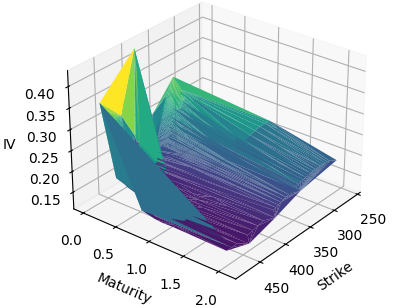
\includegraphics[width=6.5cm]{images/linear_1}
    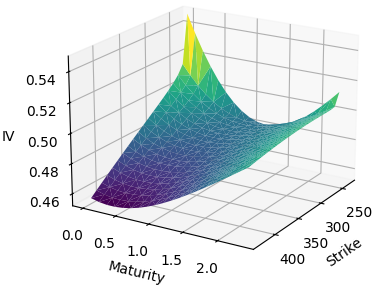
\includegraphics[width=6.5cm]{images/implicit_1}

    % Second row
    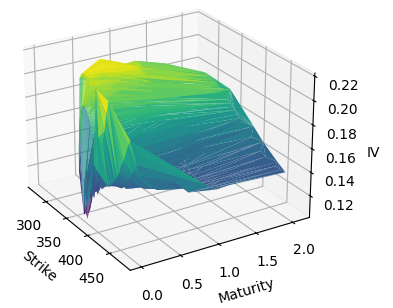
\includegraphics[width=6.5cm]{images/linear_2}
    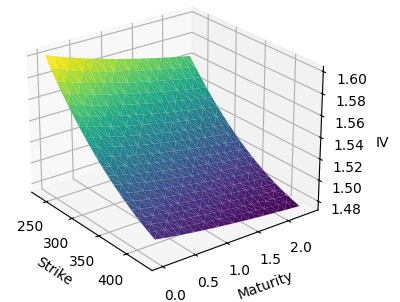
\includegraphics[width=6.5cm]{images/implicit_2}

    % Third row
    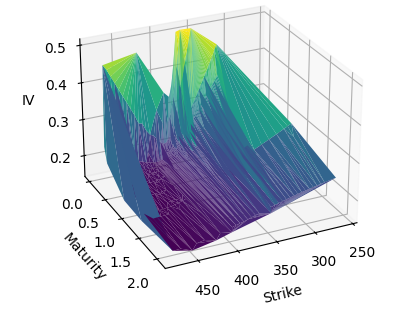
\includegraphics[width=6.5cm]{images/linear_3}
    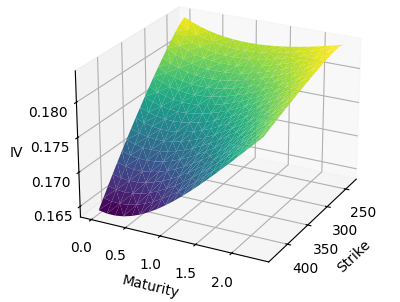
\includegraphics[width=6.5cm]{images/implicit_3}

    \caption{Surfaces interpolated on test data using a linear interpolation model (left) compared to the SABR models
    fitted with the candidate set selected using the trained implicit transformer architecture (right).}
    \label{fig:surface_comparison}
\end{figure*}

The mean train and test losses using LOO cross-validation are shown in \Cref{tab:training},
while the individual loss curves for each of the individual selector networks responsible for the $f_{\alpha}$, $f_{\rho}$, and $f_{\nu}$
functions are shown in \Cref{fig:losses}.
The execution times shown below in \Cref{tab:performance} reflect the wall time for testing on the entire dataset and on one single trading day (data point)\footnote{
    We were unable to determine why the wall time for testing on the entire dataset was $229.1$ms,
    noticeably higher than the expected $68 \times 2\text{ms} = 136\text{ms}$,
    but we attributed this difference to accumulated overhead associated with sending and retrieving data from the GPU multiple times.
}.
The obtained RMSE values for the test data show that the model was able to generalize well to the test data, with the lowest RMSE value for the $\rho$ parameter.

\begin{table}[!ht]
    \centering
    \begin{tabular}{|l|l|l|l|}
        \hline
        Metric                           & Mean time & Standard Deviation \\ \hline
        Execution time on entire dataset & 229.1ms   & 41.2ms             \\ \hline
        Execution time per point         & 2ms       & 1ms                \\ \hline
    \end{tabular}%
    \captionsetup{skip=10pt} % Adjust the caption margin
    \caption{Model performance}
    \label{tab:performance}
\end{table}